\chapter{計算機における数値の表現と誤差について}
\label{chap:基礎知識1}
一般的に,浮動小数点の方が表現できる範囲が広く計算の誤差が少ないと考えられている.
そのため,多くの計算機で浮動小数点が用いられている.
しかし,固定小数点の方が誤差が小さいような状況があれば,その状況下においては固定小数点も実用的であると考える.
そこで,本章では固定小数点と浮動小数点についての表現の違いにより,誤差が異なることを説明する.

\section{浮動小数点数と固定小数点数の表現方法}
\label{sec:bg_float_fixed}
計算機内部で扱う数値には二つの表現方法がある.
それぞれの表現方法を固定小数点数と浮動小数点数という.
これらの表現方法について説明する.
固定小数点数,浮動小数点数を説明するために,いくつかの記号を導入する.
実数全体の集合,整数全体の集合,自然数全体の集合はそれぞれ$ \R, \Z, \N$と表すのに対して,計算機の中で表現できる数全体の集合を$\mathbb{F} \ (\subset \R)$と表す.
特に,固定小数点全体の集合,浮動小数点全体の集合はそれぞれ$\fixnum,\flonum$と表す.



\subsection{固定小数点}
固定小数点数は,与えられたbit数に対して,そのうち小数部にいくつのbitを割り当てるのかを決めて残りのbitを整数部に割り当てて数を表現する方法である.
例として,$N \in \N$として計算機の中で$N$bitが数字を記憶するために与えられているとする.
そのうち,$m \ (m < N)$bitを小数部に割り当てた固定小数点数$a = a_{N-m-1} a_{N-m-2} \cdots a_1 a_0. a_{-1} \cdots a_{-m} \ (\in \fixnum)$の値は,符号を考えない場合は以下のようになる:

\begin{align*}
    a =& a_{N-m-1} 2^{N-m-1} + a_{N-m-2} 2^{N-m-2} + \cdots + a_1 2^1 + a_0 2^0 \\
    & + a_{-1} 2^{-1} + \cdots + a_{-m} 2^{-m}.
\end{align*}
ただし,$a_{i} \ (i = N-m-1,N-m-2,\dots,1,0,-1,\dots,-m)$は$0$または$1$の値を取る.
\begin{figure}[H]
    \centering
    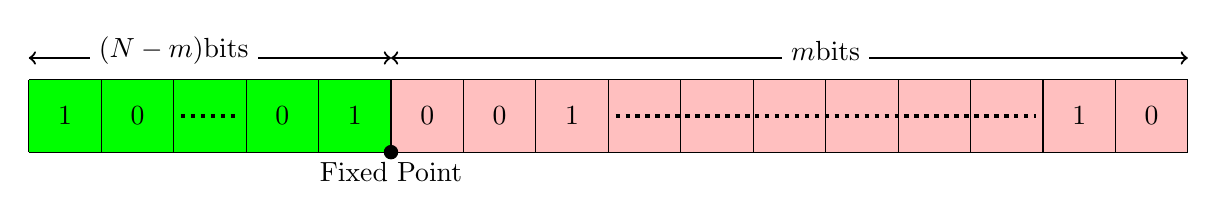
\begin{tikzpicture}[scale=0.92]
        \fill[green] (0,0) rectangle (5,1);
        \fill[pink] (5,0) rectangle (16,1);
        \draw (0,0) grid (16,1);
        \fill (5,0) circle [radius=0.1] node [below] {Fixed Point};
        \draw[ultra thick, dotted] (2.1,0.5) -- (2.9,0.5);
        \node [anchor=center] at (0.5,0.5) {1};
        \node [anchor=center] at (1.5,0.5) {0};
        \node [anchor=center] at (3.5,0.5) {0};
        \node [anchor=center] at (4.5,0.5) {1};
        \node [anchor=center] at (5.5,0.5) {0};
        \node [anchor=center] at (6.5,0.5) {0};
        \node [anchor=center] at (7.5,0.5) {1};
        \draw[ultra thick, dotted] (8.1,0.5) -- (13.9,0.5);
        \node [anchor=center] at (14.5,0.5) {1};
        \node [anchor=center] at (15.5,0.5) {0};
        \draw[<->,thick] (0,1.3) -- (5,1.3);
        \draw (2,1.4) node[fill=white] {$\small (N-m)$bits};
        \draw[<->,thick] (5,1.3) -- (16,1.3);
        \draw (11,1.4) node[fill=white] {$m$bits};
    \end{tikzpicture}
    \caption{$N$bitの符号なし固定小数点のイメージ図.}
    \label{fig:fixedpointnumber_unsigned}
\end{figure}
また,符号付き固定小数点の場合,符号に$1$bit割り当てるため整数部が$N-m-1$bitとなる.
$s$を符号とすると,符号付き固定小数点数$a_{\mathrm{signed}} = s a_{N-m-2} a_{N-m-3} \cdots a_1 a_0. a_{-1} \cdots a_{-m} \ (\in \fixnum)$の値は以下のようになる:
\begin{align*}
    a_{\mathrm{signed}} =& (-1)^s \left( a_{N-m-2} \times 2^{N-m-2} + a_{N-m-3} \times 2^{N-m-3} + \cdots \right. \\
     &\left. + a_{1} \times + 2^{1} + a_{0} \times 2^{0}+ a_{-1} \times 2^{-1} +  \cdots + a_{-m} \times 2^{-m} \right).
\end{align*}
\begin{figure}[H]
    \centering
    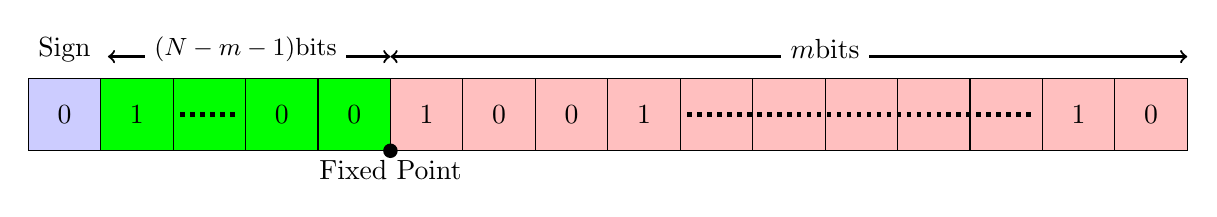
\begin{tikzpicture}[scale=0.92]
        \fill[green] (1,0) rectangle (5,1);
        \fill[pink] (5,0) rectangle (16,1);
        \fill[blue, opacity=0.2] (0,0) rectangle (1,1);
        \draw (0,0) grid (16,1);
        \fill (5,0) circle [radius=0.1] node [below] {Fixed Point};
        \draw[ultra thick, dotted] (2.1,0.5) -- (2.9,0.5);
        \node [anchor=center] at (0.5,0.5) {0};
        \node [anchor=center] at (1.5,0.5) {1};
        \node [anchor=center] at (3.5,0.5) {0};
        \node [anchor=center] at (4.5,0.5) {0};
        \node [anchor=center] at (5.5,0.5) {1};
        \node [anchor=center] at (6.5,0.5) {0};
        \node [anchor=center] at (7.5,0.5) {0};
        \node [anchor=center] at (8.5,0.5) {1};
        \draw[ultra thick, dotted] (9.1,0.5) -- (13.9,0.5);
        \node [anchor=center] at (14.5,0.5) {1};
        \node [anchor=center] at (15.5,0.5) {0};
        \draw[<->,thick] (1.1,1.3) -- (5,1.3);
        \draw[<->,thick] (5,1.3) -- (16,1.3);
        \draw (3,1.4) node[fill=white,font=\small] {$(N-m-1)$bits};
        \draw (11,1.4) node[fill=white] {$m$bits};
        \draw (0.5,1.4) node[fill=white] {Sign};
    \end{tikzpicture}
    \caption{$N$bitの符号付き固定小数点のイメージ図.}
    \label{fig:fixedpointnumber_signed}
\end{figure}
本論文では,$N$bitの符号付き固定小数点で小数部に$m$bit,整数部に$(N-m-1)$bitを割り当てた固定小数点を,
\begin{equation}
    \text{Q}(N-m-1)\text{f}m
\end{equation}
と表す.
例えば,Q11f52は符号に1bit,小数部に52bit,整数部に11bitを割り当てた固定小数点数のことを表す.
また,以降は小数部を固定した特定の固定小数点全体の集合を$\fixnumcustom{11}{52}$などと表すこととする.

\subsection{浮動小数点}
浮動小数点は,与えられたbit数に対して,bitを仮数部と指数部にわけて数を表現する方法である.
仮数部の数を$m \ (\in \Z)$,指数部の数を$e \ (\in \Z)$とすると浮動小数点$b \ (\in \flonum)$は,以下の様に表現できる:
\begin{align*}
    b = m \times 2^e.
\end{align*}
ここで$m,e$はともに2進数の数である.
浮動小数点については,国際的な規格があり,割り当てられるbit数が32bit,64bitのものをそれぞれ単精度浮動小数点(Float32),倍精度浮動小数点(Float64)という.
それぞれの浮動小数点数の仮数部と指数部のbit数は以下の表のように決められている:
\begin{table}[H]
    \centering
    \caption{単精度浮動小数点(Float32)と倍精度浮動小数点(Float64)の仮数部と指数部のbit数.}
    \begin{tabular}{c|c|c}   
     & 仮数部 & 指数部 \\ \hline
    Float32 & 23bit & 8bit \\ 
    Float64 & 52bit & 11bit
    \end{tabular}
    \label{tab:Float32_Float64_bit}
\end{table}
以降,単精度浮動小数点全体の集合,倍精度浮動小数点全体の集合を$\floatsigle,\floatdouble$などと表すこととする.
単精度浮動小数点(Float32)の割り当ては以下の様になる:
\begin{figure}[H]
    \centering
    \begin{tikzpicture}[scale=0.92]
        \fill[green] (1,0) rectangle (5,1);
        \fill[pink] (5,0) rectangle (16,1);
        \fill[blue, opacity=0.2] (0,0) rectangle (1,1);
        \draw (0,0) grid (16,1);
        \draw[ultra thick, dotted] (2.1,0.5) -- (2.9,0.5);
        \node [anchor=center] at (0.5,0.5) {0};
        \node [anchor=center] at (1.5,0.5) {1};
        \node [anchor=center] at (3.5,0.5) {0};
        \node [anchor=center] at (4.5,0.5) {0};
        \node [anchor=center] at (5.5,0.5) {1};
        \node [anchor=center] at (6.5,0.5) {0};
        \node [anchor=center] at (7.5,0.5) {0};
        \node [anchor=center] at (8.5,0.5) {1};
        \draw[ultra thick, dotted] (9.1,0.5) -- (13.9,0.5);
        \node [anchor=center] at (14.5,0.5) {1};
        \node [anchor=center] at (15.5,0.5) {0};
        \draw[<->,thick] (1.1,1.3) -- (5,1.3);
        \draw[<->,thick] (5,1.3) -- (16,1.3);
        \draw (3,1.4) node[fill=white] {指数部$8$bits};
        \draw (11,1.4) node[fill=white] {仮数部$23$bits};
        \draw (0.5,1.4) node[fill=white] {Sign};
    \end{tikzpicture}
    \caption{単精度浮動小数点(Float32)のイメージ図.}
    \label{fig:float32_bit}
\end{figure}
単精度浮動小数点(Float32)は,指数部の8bitで整数値では$0 \sim  255$の値を取るが$-127$のバイアスがある.
つまり,実際の指数部の数は計算機内で表せる2進数の数から$127$を引いた数となっている.
また,仮数部の値は暗黙に一つ上の位が$1$であるとして,小数点以下の位を表す表現方法を用いている.
よって,単精度浮動小数点で表せられる値$b_{32} \ (\in \floatsigle)$は,指数部の数を$e_{32}$,仮数部の各bitを$b_{-1}$,$b_{-2}$,...,$b{-23}$とすると,
\begin{align*}
    b_{32} &= (-1)^{\mathrm{sign}}(1 + b_{-1}\times 2^{-1} + b_{-2}\times 2^{-2} + \cdots + b_{-23}\times 2^{-23})\times 2^{e_{32} - 127} \\
        &= (-1)^{\mathrm{sign}}\left(1 + \sum_{i = 1}^{23} b_{-i} 2^{-i}\right)\times 2^{e_{32} - 127}
\end{align*}
となる.
倍精度浮動小数点(Float64)の割り当ては以下の様になる:
\begin{figure}[H]
    \centering
    \begin{tikzpicture}[scale=0.92]
        \fill[green] (1,0) rectangle (5,1);
        \fill[pink] (5,0) rectangle (16,1);
        \fill[blue, opacity=0.2] (0,0) rectangle (1,1);
        \draw (0,0) grid (16,1);
        \draw[ultra thick, dotted] (2.1,0.5) -- (2.9,0.5);
        \node [anchor=center] at (0.5,0.5) {0};
        \node [anchor=center] at (1.5,0.5) {1};
        \node [anchor=center] at (3.5,0.5) {0};
        \node [anchor=center] at (4.5,0.5) {0};
        \node [anchor=center] at (5.5,0.5) {1};
        \node [anchor=center] at (6.5,0.5) {0};
        \node [anchor=center] at (7.5,0.5) {0};
        \node [anchor=center] at (8.5,0.5) {1};
        \draw[ultra thick, dotted] (9.1,0.5) -- (13.9,0.5);
        \node [anchor=center] at (14.5,0.5) {1};
        \node [anchor=center] at (15.5,0.5) {0};
        \draw[<->,thick] (1.1,1.3) -- (5,1.3);
        \draw[<->,thick] (5,1.3) -- (16,1.3);
        \draw (3,1.4) node[fill=white] {指数部$11$bits};
        \draw (11,1.4) node[fill=white] {仮数部$52$bits};
        \draw (0.5,1.4) node[fill=white] {Sign};
    \end{tikzpicture}
    \caption{倍精度浮動小数点(Float64)のイメージ図.}
    \label{fig:float64_bit}
\end{figure}
倍精度浮動小数点(Float64)は指数部の11bitで整数値では$0 \sim  2047$の値を取るが$-1023$のバイアスがある.
また,単精度浮動小数点と同様に仮数部の値は暗黙に一つ上の位が$1$であるとして,小数点以下の位を表す表現方法を用いている.
よって,倍精度浮動小数点で表せられる値$b_{64} \ (\in \floatdouble)$は,指数部の数を$e_{64}$,仮数部の各bitを$b_{-1}$,$b_{-2}$,...,$b{-52}$とすると,
\begin{align*}
    b_{64} &= (-1)^{\mathrm{sign}}(1 + b_{-1}\times 2^{-1} + b_{-2}\times 2^{-2} + \cdots + b_{-52}\times 2^{-52})\times 2^{e_{64} - 1023} \\
        &= (-1)^{\mathrm{sign}}\left(1 + \sum_{i = 1}^{52} b_{-i} 2^{-i}\right)\times 2^{e_{64} - 1023}
\end{align*}
となる.
以上から浮動小数点はbit数によって表現出来る数の範囲が異なる.
単精度浮動小数点と倍精度浮動小数点では以下の様になる:
\begin{table}[H]
    \centering
        \caption{単精度浮動小数点と倍精度浮動小数点の表現可能な数の範囲.}
        \small
        \begin{tabular}{p{3em}|>{\centering}p{11em}|>{\centering}p{11em}|c}   
            & 最大値 & 最小 & 0に最も近い数 \\ \hline \hline
            {\scriptsize Float32} &
            \begin{tabular}{c}
                ${\scriptsize\sum_{i=105}^{128}2^i}$ \\
                ${\scriptsize\backsimeq 3.402824\times 10^{38}}$
            \end{tabular}&
            \begin{tabular}{c}
                ${\scriptsize-\sum_{i=105}^{128}2^i}$ \\
                ${\scriptsize\backsimeq -3.402824\times 10^{38}}$
            \end{tabular}&
            \begin{tabular}{c}
                ${\scriptsize2^{-127}}$ \\
                ${\scriptsize\backsimeq 1.175494\times 10^{-38}}$
            \end{tabular} \\ \hline
            {\scriptsize Float64} &
            \begin{tabular}{c}
                ${\scriptsize\sum_{i=927}^{1024}2^i}$ \\
                ${\scriptsize\backsimeq 1.797693\times 10^{308}}$
            \end{tabular}&
            \begin{tabular}{c}
                ${\scriptsize-\sum_{i=927}^{1024}2^i}$ \\
                ${\scriptsize\backsimeq -1.797693\times 10^{308}}$
            \end{tabular}&
            \begin{tabular}{c}
                ${\scriptsize2^{-1023}}$ \\
                ${\scriptsize\backsimeq 2.225074\times 10^{-308}}$
            \end{tabular}
        \end{tabular}
        \label{tab:Float32_Float64_range}
\end{table}

以上のように,固定小数点数と浮動小数点数には表現出来る数の範囲や0に最も近い値に違いある.
そのイメージを表したのが以下の図である.
\begin{figure}[H]
    \centering
    \begin{tikzpicture}
        \draw [->, thick] (-7,0) -- (7,0);
        \draw [thick] (-6,0.2) -- (-6,-0.2);
        \draw [thick] (-5,0.2) -- (-5,-0.2);
        \draw [thick] (-4,0.2) -- (-4,-0.2);
        \draw [thick] (-3,0.2) -- (-3,-0.2);
        \draw [thick] (-2,0.2) -- (-2,-0.2);
        \draw [thick] (-1,0.2) -- (-1,-0.2);
        \draw [thick] (0,0.5) -- (0,-0.5) node [below] {0};
        \draw [thick] (1,0.2) -- (1,-0.2);
        \draw [thick] (2,0.2) -- (2,-0.2);
        \draw [thick] (3,0.2) -- (3,-0.2);
        \draw [thick] (4,0.2) -- (4,-0.2);
        \draw [thick] (5,0.2) -- (5,-0.2);
        \draw [thick] (6,0.2) -- (6,-0.2);
    \end{tikzpicture}
    \caption{固定小数点数の値として表せる数のイメージ図.横線が数直線,縦線が表現出来る数を示す.}
    \label{fig:fixedpoint_image}
\end{figure}

\begin{figure}[H]
    \centering
    \begin{tikzpicture}
        \draw [->, thick] (-7,0) -- (7,0);
        \draw [thick] (-4,0.2) -- (-4,-0.2);
        \draw [thick] (-2,0.2) -- (-2,-0.2);
        \draw [thick] (-1,0.2) -- (-1,-0.2);
        \draw [thick] (-0.5,0.2) -- (-0.5,-0.2);
        \draw [thick] (-0.25,0.2) -- (-0.25,-0.2);
        \draw [thick] (-0.125,0.2) -- (-0.125,-0.2);
        \draw [thick] (0,0.5) -- (0,-0.5) node [below] {0};
        \draw [thick] (0.125,0.2) -- (0.125,-0.2);
        \draw [thick] (0.25,0.2) -- (0.25,-0.2);
        \draw [thick] (0.5,0.2) -- (0.5,-0.2);
        \draw [thick] (1,0.2) -- (1,-0.2);
        \draw [thick] (2,0.2) -- (2,-0.2);
        \draw [thick] (4,0.2) -- (4,-0.2);
    \end{tikzpicture}
    \caption{浮動小数点数の値として表せる数のイメージ図.横線が数直線,縦線が表現出来る数を示す.}
    \label{fig:floatpoint_image}
\end{figure}
図\ref{fig:fixedpoint_image}のように固定小数点数で表せる数で隣り合う数は隣の数までの間隔が一定である.
それに対して図\ref{fig:floatpoint_image}のように浮動小数点数で表せる数で隣り合う数は隣の数までの間隔が一定ではない.
浮動小数点数で表せる数で2つの隣り合う数は,$0$に近い値ほど間隔が小さく密になり,$0$から離れるほど指数的に大きくなる.

図\ref{fig:fixedpoint_image},\ref{fig:floatpoint_image}で表したように,固定小数点,浮動小数点ともに計算機の中で表すことのできる数は限られている.

\section{浮動小数点と固定小数点の演算方法}
\label{sec:float_fixed_expression}
\begin{comment}
    ストーリー:
    固定小数点演算は浮動小数点演算よりも計算時間が速いとされている.<-これいらないかも
    しかし,浮動小数点に比べて精度が低くなる恐れがある.
    本論文では,固定小数点と浮動小数点での数値計算の結果を比べ,固定小数点での演算も浮動小数点と同程度の精度で計算できることを示した.
    実験結果より固定小数点演算で浮動小数点より高速で,浮動小数点と同程度の計算を実現できるのではないかと考える.
\end{comment}
本論文で行う実験は,数値計算を固定小数点によって計算することである.
本章では,固定小数点と浮動小数点の表現できる数の範囲や扱える数の最小単位の大きさ,演算の違いについて述べる.
第\ref{sec:bg_float_fixed}章で述べたように,固定小数点と浮動小数点では表現方法が異なる.
そのため,固定小数点と浮動小数点には数値を表現する上での利点と欠点が存在する.
第\ref{sec:float_fixed_expression}章では,固定小数点と浮動小数点の表現方法と演算方法についての利点と欠点を述べる.

\subsection{固定小数点と浮動小数点の表現範囲と数の最小単位}
固定小数数点と浮動小数点では,表現方法が異なるためそれぞれに利点が存在する.
浮動小数点の利点は,表現できる数の範囲が同じbit数の固定小数点よりも広いことである.
例として,同じ64bitの固定小数点と倍精度浮動小数点(Float64)を考える.
表\ref{tab:fixed_float_range}は,固定小数点と浮動小数点の表現できる数の範囲を示したものである.

\begin{table}[H]
    \centering
    \caption{固定小数点(Q11f52,Q62f1)と浮動小数点(Float64)の表現できる数の範囲}
    \begin{tabular}{c|c|c}
         & 最小値 & 最大値 \\ \hline\hline
          Float64 & $-1.798 \times 10^{308}$ & $1.798 \times 10^{308}$ \\
          Q11f52 & $-2048$ & $2048$ \\
          Q62f1 & $-4.612 \times 10^{18}$ & $-4.612 \times 10^{18}$
    \end{tabular}
    \label{tab:fixed_float_range}
\end{table}

表\ref{tab:fixed_float_range}で示したのは倍精度浮動小数点(Float64)と,小数部のbit数が倍精度浮動小数点(Float64)の仮数部と同じbit数の固定小数点(Q11f52)と64bitの固定小数点のうち表現できる数の範囲が最大の固定小数点(Q62f1)の表現できる数の範囲である.
この表から分かるように,浮動小数点の方が表現できる数の範囲が固定小数点に比べとても大きい.
数値計算を行う際に,計算の過程で扱う数が計算機で扱う数の範囲を超えてしまうオーバーフローという現象が発生する心配がある.
浮動小数点は,固定小数数点に比べ表現できる数の範囲が広いため,固定小数点に比べオーバーフローが起こりにくいという利点がある.

次に,固定小数点と浮動小数点の扱える数の最小単位について述べる.
第\ref{chap:基礎知識2}で述べたように,固定小数点は小数点が固定されているため最小単位の値によらず一定であるのに対して,浮動小数点の最小単位の値の指数部の大きさによって異なる.

表\ref{tab:fixed_float_zero_error}は固定小数点(Q11f52,Q1f62)と浮動小数点(Float64)の$0$に最も近い値を示したものである.

\begin{table}[H]
    \centering
    \caption{固定小数点(Q11f52,Q1f62)と浮動小数点(Float64)の$0$に最も近い値}
    \begin{tabular}{c|c}
        & $0$に最も近い数 \\ \hline \hline
        Float64 & $2.225 \times 10^{-308}$\\
        Q11f52  & $2.220 \times 10^{-16}$\\
        Q1f62   & $2.168 \times 10^{-19} $
    \end{tabular}
    \label{tab:fixed_float_zero_error}
\end{table}

このように,浮動小数点は絶対値のとても小さい数も表現できるため,固定小数点に比べアンダーフローを起こしにくいという利点がある.

\subsection{浮動小数点と固定小数点の演算の違い}
\label{sec:dif_arithmetic}
\begin{comment} %今回の論文は速さについては言及してない.   
    計算機の中で主に演算を行うのはCPU(Central Processing Unit)である.
    固定小数点と浮動小数点では,演算におけるCPUへの負担が異なり浮動小数点の方が負荷が大きい.
    そのため,かつてはCPUの性能が低く浮動小数点を専門に扱うためのFPU(Floating Point Unit)を用いて浮動小数点演算を行なっていた.
    現代では,CPUの性能が向上したためFPUの機能はCPU自体に組み込まれていることが多い.
    しかし,浮動小数点演算を組み込まずに固定小数点演算を行うような計算機があれば,計算の負荷を少なくすることが可能である.
    以下では,固定小数点と浮動小数点の演算の違いについて述べる.
\end{comment}
固定小数点と浮動小数点は,数の表現方法の違いから四則演算の方法が異なる.
固定小数点は厳密な四則演算と似たように加減算が行えるのに対して,浮動小数点は指数部の大きさを揃えてから加減算を行わなければいけないといった違いがある.
第\ref{sec:dif_arithmetic}では,固定小数点と浮動小数点の四則演算の違いについて述べる.

\subsubsection{固定小数点の演算}
固定小数数点の四則演算は,整数での四則演算と同様に行える.
例えば,整数部が3bitで小数部が4bitの符号あり固定小数点$\fixnumcustom{3}{4}$の四則演算を行う場合を考える.
2数$0010.1101_{\fixnumcustom{3}{4}} \ (= 2.8125)$と$0010.1110_{\fixnumcustom{3}{4}} \ (= 2.875)$の加法を行う場合,2数に小数部と同じbit数分だけ2をかける.
つまり,2数を$2^4$倍して,整数$00101101_{(2)}$と$00101110_{(2)}$を加算することで,整数同士の演算を行い,その計算結果を最初にかけた数でわることで結果を求めることができる.
数式で表すと式\eqref{eq:fixed_add_first}〜\eqref{eq:fixed_add_last}のようになる.
\begin{align}
    2.8125 + 2.875 &=
    0010.1101_{(2)} + 0010.1110_{(2)} \label{eq:fixed_add_first} \\
    &= \left\{ 2^4 \times \left(0010.1101_{(2)} + 0010.1110_{(2)}\right) \right\} \div 2^4 \\
    &= \left(00101101_{(2)} + 00101110_{(2)} \right) \div 2^4= 01011011_{(2)} \div 2^4\\
    &= 91 \div 2^4 = 5.6875 \label{eq:fixed_add_last}
\end{align}

数式での厳密な四則演算を$+,-,\times,\div$,計算機内の四則演算を$\fixadd,\fixsub ,\fixmul,\\ \fixdiv$と表すことにする.
また,2数の演算結果も数値型の表せる範囲内であるのもとし,実数$a$に対して計算機で$a$を表す数を$a^{\ast}$とする.
加法と減法については,数式と同じように行うことができ,$a+b$,$a-b$を計算機で行うと,
\begin{align*}
    a^{\ast} \fixadd b^{\ast} &= a^{\ast} + b^{\ast}, \\ 
    a^{\ast} \fixsub b^{\ast} &= a^{\ast} - b^{\ast}
\end{align*}
となる.
乗法については,数式で厳密な計算を行うと$m$桁の数と$m$桁の数同士の乗法の演算結果は最大で$2m$桁になるため,表現が可能な小数部のbit数までで打ち切る.
$a \times b$を計算機内で行うと,
\begin{align*}  
    a^{\ast} \fixmul b^{\ast} = \left(a^{\ast} \times b^{\ast}\right)^{\ast}
\end{align*}
となる.
例として,$0000.0011_{(2)} \in \fixnumcustom{3}{4}$と$0001.0001_{(2)} \in \fixnumcustom{3}{4}$の乗法を考えると,
\begin{align*}
    0000.0011_{(2)} \fixmul 00001.0001_{(2)} &= \left(0000.0011_{(2)} \times 0001.0001_{(2)}\right)^{\ast} \\
    &= \left(0001.10011\right)^{\ast} = 0001.1010_{(2)}
\end{align*}
となる.


除法については,数式での厳密な計算では,割り切れないこともあり商が循環小数となる場合もある.
そのため,乗算の場合と同じく表現できる小数部のbit数までで打ち切る.
$a \div b$を計算機内で行うと,
\begin{align*}
    a^{\ast} \fixdiv b^{\ast} = \left(a^{\ast} \div b^{\ast}\right)^{\ast}
\end{align*}
となる.
例として,$0001.0000_{(2)} \in \fixnumcustom{3}{4}$と$0011.0000_{(2)} \in \fixnumcustom{3}{4}$の除法を考えると,
\begin{align*}
    0001.0000_{(2)} \fixdiv 0011.0000_{(2)} &= \left(0001.0000_{(2)} \div 0011.0000_{(2)}\right)^{\ast} \\
    &= \left(0000.0101010_{(2)}\dots\right)^{\ast} = 0000.0101_{(2)}
\end{align*}
となる.


固定小数点の乗算,除算では表現できる小数部のbit数までで打ち切るため,誤差が発生するが基本的な演算は数式での四則演算と同じである.

\subsubsection{浮動小数点の演算}
浮動小数点は,与えられたbit数を仮数部と指数部という二つの部分に分けて表現するため,四則演算を行うときに注意が必要である.
$p$進数の浮動小数点は,指数部を$e$,仮数部を$m$としたとき,
\begin{align*}
    m \times p^e
\end{align*}
と表現される.
ただし,$1 \leq m < p$とする.
通常の計算機では2進数で表現されるが,説明のため10進数の表\ref{tab:float_setting}で定めた浮動小数点を扱うことにする.
\begin{table}[H]
    \centering
    \caption{説明で用いる浮動小数点の設定.}
    \begin{tabular}{ccc}
        \hline
        $p=10$ & & \\
        指数部$e$ & 最大値$10$ & 最小値$-10$ \\
        仮数部$m$ & 4桁 &
    \end{tabular}
    \label{tab:float_setting}
\end{table}

数式での厳密な四則演算を$+,-,\times,\div$とし,計算機内での四則演算を$\floadd,\flosub,\floomul,\flodiv$と表すことにする.

実数$a$に対して計算機内で$a$を表す数を$a^{\ast}$とし,$a^{\ast}$の指数部を$e_{a^{\ast}}$,仮数部を$m_{a^{\ast}}$とする.
行う手順については,計算機の使用などによって順番は異なる場合もあるが捜査としては同じことを行う.


加法については,$a + b$を計算機で行う手順は,
\begin{enumerate}
    \item 指数部$e_{a^{\ast}}$と$e_{b^{\ast}}$を比較し,仮数部$m_{a^{\ast}}$と$m_{b^{\ast}}$の位を揃える.
    \item 位を揃えた仮数部$m_{a^{\ast}}$と$m_{b^{\ast}}$を加算する.
    \item 位を揃えた仮数部の計算結果をもとに,計算結果の指数部と仮数部を決める.
\end{enumerate}
となる.
例として,$1.234 \times 10^{-1}$と$2.356 \times 10^{2}$の加法を行うと,
\begin{align*}
    1.234 \times 10^{-1} \floadd 2.356 \times 10^{2} &= 0.1235 + 235.6 \\
    &= 235.7235 
    &\simeq 2.357 \times 10^{2}
\end{align*}
となる.

減法については,$a - b$を計算機で行う手順は,
\begin{enumerate}
    \item 指数部$e_{a^{\ast}}$と$e_{b^{\ast}}$を比較し,仮数部$m_{a^{\ast}}$と$m_{b^{\ast}}$の位を揃える.
    \item 位を揃えた仮数部$m_{a^{\ast}}$と$m_{b^{\ast}}$を減算する.
    \item 位を揃えた仮数部の計算結果をもとに,計算結果の指数部と仮数部を決める.
\end{enumerate}
となる.

乗算については,$a \times b$を計算機で行う手順は,
\begin{enumerate}
    \item 指数部$e_{a^{\ast}}$と$e_{b^{\ast}}$を加算する.
    \item 仮数部$m_{a^{\ast}}$と$m_{b^{\ast}}$の乗算を行う.
    \item 仮数部の計算結果を指数部に反映させて計算結果の指数部と仮数部を決める.
    \item 符号を調整する.
\end{enumerate}
となる.
例として,$2.435 \times 10^2$と$5.100 \times 10^4$の乗法を行うと,指数部の計算は
\begin{align*}
    2 + 4 = 6
\end{align*}
であり,仮数部の計算は,
\begin{align*}
    2.435 \times 5.100 = 12.4185
\end{align*}
であるので,そのまま計算を行うと$12.4185 \times 10^6$となるが,指数部と仮数部の数を調整して,
\begin{align*}
    2.435 \times 10^2 \floomul 5.100 \times 10^4 &= 1.242 \times 10^6
\end{align*}
となる.

除法については,$a \div b$を計算機で行う手順は,
\begin{enumerate}
    \item 指数部$e_{a^{\ast}}$と$e_{b^{\ast}}$を減算する.
    \item 仮数部$m_{a^{\ast}}$と$m_{b^{\ast}}$の除算を行う.
    \item 仮数部の計算結果を指数部に反映させて計算結果の指数部と仮数部を決める.
    \item 符号を調整する.
\end{enumerate}
となる.
例として,$1.000 \times 10^5$と$3.000 \times 10^7$の除法を行うと,指数部の計算は,
\begin{align*}
    5 - 7 = -2
\end{align*}
であり,仮数部の計算は,
\begin{align*}
    1.000 \div 3.000 = 0.33333\dots
\end{align*}
であるので,そのまま計算を行うと$0.33333\dots \times 10^{-2}$となるが,指数部と仮数部の数を調整して,
\begin{align*}
    1.000 \times 10^5 \flodiv 3.000 \times 10^7 &= 3.333 \times 10^{-3}
\end{align*}
となる.

\section{丸め誤差・情報落ち・桁落ちについての基礎知識}
第\ref{}節で述べたように計算機の中では表現できる数に限りがある.
そのため計算機の中で表現できる数はそのままの数で計算を行うが,計算機の中で表現できない数はその数にできるだけ近い表現をできる数を代わりに用いて計算を行うことになる.
ある数$a\ \in \R$に対して,計算機で$a$という数を扱う場合の表現を
\begin{equation*}    
    a^{\ast} \ (\in \mathbb{F})
\end{equation*}
とする.
また,$a$を$p$進数で表現することを明記する場合,
\begin{equation*}
    a_{(p)}
\end{equation*}
と表すことにする.
\label{chap:基礎知識2}

\subsection{丸め誤差}
丸め誤差について説明する.
丸め誤差とは,真の値と計算機で表現するために代わりに用いる数の差である.
真の値を$x_{\mathrm{true}} \ (\in \R)$とする.
計算機の中で表現できる数で$x_{\mathrm{true}}$に一番近い数を$x^{\ast} \ (\in \mathbb{F})$とすると,そのときの丸め誤差$\rounderror$は,
\begin{equation*}
    \rounderror = x_{\mathrm{true}} - x^{\ast}
\end{equation*}
と表せる.
簡単のため,計算機で扱われる2進数ではなく10進数を用いた場合を考える.
例えば,計算機では,小数点2桁までしか表現できないとすると,$\pi$という数は,計算機の中で
\begin{equation*}
    \pi^{\ast}_{(10)} = 3.14_{(10)} \ (\in \mathbb{F})
\end{equation*}
という数で扱うことになる.
そして,丸め誤差$e_{\mathrm{round}}$は,
\begin{equation*}
    {\rounderror}_{(10)} = \pi - \pi^{\ast} = {0.00159265_{(10)}\dots}
\end{equation*}
となる.


次に,丸め誤差の大きさがどの程度であるかについて述べる.
$a \in \R$を計算機の中で表現することを考える.ただし,ここでは計算機の中で表現される数は10進数ではなく2進数であるとする.
ただし,浮動小数点で表せる最大の数を${M_{\mathrm{float}}}_{(2)}$,最小の数を${m_{\mathrm{float}}}_{(2)}$,固定小数点で表せる最大の数を${M_{\mathrm{fixed}}}_{(2)}$,最小の数を${m_{\mathrm{fixed}}}_{(2)}$とし,
\begin{align*}
   {m_{\mathrm{float}}}_{(2)} &< a_{(2)} < {M_{\mathrm{float}}}_{(2)}, \\
   {m_{\mathrm{fixed}}}_{(2)} &< a_{(2)} < {M_{\mathrm{fixed}}}_{(2)}
\end{align*}
とする.
浮動小数点での丸め誤差について述べ,続いて固定小数点の丸め誤差について述べる.
一般的な浮動小数点(Float32,Float54)では,$m_{\mathrm{float}}$,$M_{\mathrm{float}}$のおおよその値は図\ref{tab:float_max_min}のようになる.
\begin{table}[H]
    \centering
    \caption{Float32,Float64での$m_{\mathrm{float}}$と$M_{\mathrm{float}}$のおおよその値.}
    \begin{tabular}{c|c|c}
         & $m_{\mathrm{float}}$ & $M_{\mathrm{float}}$ \\ \hline \hline
         Float32 & $-3.40 \times 10^{38}$ & $3.40 \times 10^{38}$ \\ \hline
         Float64 & $-1.80 \times 10^{308}$ & $1.80 \times 10^{308}$
    \end{tabular}
    \label{tab:float_max_min}
\end{table}

丸め誤差は浮動小数点の場合,仮数部を$m$bit,指数部を$e$bitとする.
ただし,以下ではFloat32,Float64とは異なり指数部$e$にバイアスはないものとする.
$a^{\ast}_{(2)} \ (\in \flonum)$の中で,
\begin{align*}
    {a^{\ast}}_{(2)} < a_{(2)}\ \text{かつ} |a_{(2)} - {a^{\ast}}_{(2)}| \ \text{が最小}
\end{align*}
となるような数${a^{\ast}}_{(2)}$を${a^{\ast}_{\mathrm{small}}}_{(2)}$とする.
${a^{\ast}_{\mathrm{small}}}_{(2)}$の仮数部を$\mathcal{M}_{\mathrm{small}}$,指数部を$\mathcal{E}_{\mathrm{small}}$とする.
たま,
\begin{align*}
    {a^{\ast}}_{(2)} > a_{(2)} \ \text{かつ} |a_{(2)} - {a^{\ast}}_{(2)}| \ \text{が最小}
\end{align*}
となるような数${a^{\ast}}_{(2)}$を${a^{\ast}_{\mathrm{large}}}_{(2)}$とする.
${a^{\ast}_{\mathrm{large}}}_{(2)}$の仮数部を$\mathcal{M}_{\mathrm{large}}$,指数部を$\mathcal{E}_{\mathrm{large}}$とする.
このとき,
\begin{align*}
    |a - {a^{\ast}_{\mathrm{sall}}}_{(2)}| &\leq 2^{-m+{\expparts}}, \\
    |a - {a^{\ast}_{\mathrm{large}}}_{(2)}| &\leq 2^{-m+{\expparts}}
\end{align*}
であり,$a^{\ast}_{(2)}$が
\begin{align*}
    2^{\beta -1} < a^{\ast}_{(2)} < 2^{\beta}
\end{align*}
となるとき,
\begin{equation*}
    \mathcal{E}_{\mathrm{small}} = \mathcal{E}_{\mathrm{large}} = \beta
\end{equation*}
である.$a^{\ast}_{(2)}$は
\begin{align*}
    {a^{\ast}}_{(2)} = \left\{ 
        \begin{array}{ll}
            {a^{\ast}_{\mathrm{small}}}_{(2)} &\text{if} \ |a^{\ast}_{2} - {a^{\ast}_{\mathrm{small}}}_{(2)} | < |a^{\ast}_{2} - {a^{\ast}_{\mathrm{large}}}_{(2)} | \\
            {a^{\ast}_{\mathrm{large}}}_{(2)} &\text{if} \ |a^{\ast}_{2} - {a^{\ast}_{\mathrm{small}}}_{(2)} | \geq |a^{\ast}_{2} - {a^{\ast}_{\mathrm{large}}}_{(2)} | 
        \end{array}
    \right.
\end{align*}
となるので,丸め誤差$e_{\mathrm{round}}$は最大で
\begin{align}
    \label{eq:rounderror_float}
    |e_{\mathrm{round}}| \leq 2^{-m+\beta -1}
\end{align}
となる.
ここで,$m$は一定の値であり,$\beta$は$a^{\ast}_{(2)}$の値により決まる値である.


固定小数点の場合,小数部が$m$bitとし,${a^{\ast}}_{(2)} \ (\in\fixnum)$の中で,
\begin{align*}
    {a^{\ast}}_{(2)} < a_{(2)}\ \text{かつ} |a_{(2)} - {a^{\ast}}_{(2)}| \ \text{が最小}
\end{align*}
となるような数${a^{\ast}}_{(2)}$を${a^{\ast}_{\mathrm{small}}}_{(2)}$とする.
たま,
\begin{align*}
    {a^{\ast}}_{(2)} > a_{(2)} \ \text{かつ} |a_{(2)} - {a^{\ast}}_{(2)}| \ \text{が最小}
\end{align*}
となるような数${a^{\ast}}_{(2)}$を${a^{\ast}_{\mathrm{large}}}_{(2)}$とする.
このとき,
\begin{align}
    |a - {a^{\ast}_{\mathrm{sall}}}_{(2)}| &\leq 2^{-m}, \\
    |a - {a^{\ast}_{\mathrm{large}}}_{(2)}| &\leq 2^{-m}
\end{align}
であり,
\begin{align*}
    {a^{\ast}}_{(2)} = \left\{ 
        \begin{array}{ll}
            {a^{\ast}_{\mathrm{small}}}_{(2)} &\text{if} \ |a^{\ast}_{2} - {a^{\ast}_{\mathrm{small}}}_{(2)} | < |a^{\ast}_{2} - {a^{\ast}_{\mathrm{large}}}_{(2)} | \\
            {a^{\ast}_{\mathrm{large}}}_{(2)} &\text{if} \ |a^{\ast}_{2} - {a^{\ast}_{\mathrm{small}}}_{(2)} | \geq |a^{\ast}_{2} - {a^{\ast}_{\mathrm{large}}}_{(2)} | 
        \end{array}
    \right.
\end{align*}
となるので,丸め誤差$e_{\mathrm{round}}$は最大で
\begin{align}
    \label{eq:rounderror_fixed}
    |\rounderror| \leq 2^{-m-1}
\end{align}
となる.ここで$m$は一定の値である.


式\eqref{eq:rounderror_float},\eqref{eq:rounderror_fixed}から,固定小数点では丸め誤差取りうる値のうち最大値が$a^{\ast}_{(2)}$の値に依らず一定であるのに対して,浮動小数点では$a^{\ast}_{(2)}$の値がどのような範囲にあるのかにより丸め誤差がとりうる値のうち最大値の大きさが異なる.
表\ref{tab:fixed_float_rounding_error}は同じ64bitの倍精度浮動小数点(Float64)と倍精度浮動小数点(Float64)の仮数部と同じbit数の小数部を持つ固定小数点(Q11f52)の丸め誤差を表したものである.

\begin{table}[H]
    \centering
    \caption{固定小数点(Q11f52)と浮動小数点(Float64)のそれぞれの数値に対する丸め誤差の大きさ}
    \begin{tabular}{c|c|c}
        & Q11f52 & Float64 \\ \hline \hline
        0.01 & $8.674 \times 10^{-18}$ & $1.735 \times 10^{-18}$\\
        0.1 & $8.327 \times 10^{-17}$ & $1.388 \times 10^{-17}$\\
        1.1 & $8.327 \times 10^{-17}$ & $2.220 \times 10^{-16}$\\
        10.1 & $8.327 \times 10^{-17}$ & $1.776 \times 10^{-15}$\\
        100.1 & $8.327 \times 10^{-17}$ & $1.421 \times 10^{-14}$ 
    \end{tabular}
    \label{tab:fixed_float_rounding_error}
\end{table}

このように,固定小数点は,$1$よりも大きい数に対しては丸め誤差の値が一定であるのに対して,浮動小数点は,絶対値の小さい数に対しては丸め誤差の値も小さく,絶対値の大きい数に対しては丸め誤差の値も大きくなる.
固定小数点は,小数部のbit数が同じでありるため表現できる数の中で隣り合う2数の間隔が一定であるのに対して,浮動小数点は表現できる2数の間隔が2数の絶対値の大きさによって異なる.
そのため,固定小数点と浮動小数点では丸め誤差が真の値によって異なる.
また,数値計算において絶対値がとても小さい数を表現できなくなるアンダーフローという現象がある.


計算機で計算を繰り返し行うと,一度の計算で発生した丸め誤差が次の計算に影響を与えるため,計算回数が多くなるにつれ計算機で行われる計算の結果と厳密な計算の結果の差は大きくなる.

\subsection{打ち切り誤差}
打ち切り誤差とは,問題の真の結果と解法を用いて厳密な計算により得られる結果の差である.
以下のような微分方程式を陽的Euler法で$t \in [0,T]$の範囲で解くとこを考える:
\begin{equation*}
    \differencial{x}{t} = f(t,x(t)), \ x(0) = x_0.
\end{equation*}
Euler法は付録\ref{chap:補遺}で説明する方法である.
まず,時刻$t,t+\Delta t$における解を$x(t),x(t+\Delta t)$とし,2次の項までTaylor展開すると
\begin{align}
    \label{eq:taylor_euler}
    x(t + \Delta t) = x(t) + \frac{\delt}{1!}x^{\prime}(t) + \frac{\delt^2}{2!}x^{\prime\prime}(t + \theta\delt) \ (0 < \theta < 1)
\end{align}
である.
一方,陽的Euler法では
\begin{align}
    \label{eq:euler_appro}
    x(t + \Delta t) \backsimeq x(t) + \frac{\delt}{1!}f(t,x(t))
\end{align}
という近似により解を得るため,式\eqref{eq:taylor_euler},\eqref{eq:euler_appro}より真の解$x_{\mathrm{true}}(t)$とEuler法により得られる解$x_{\mathrm{euler}}(t)$には,
\begin{align*}
    x_{\mathrm{true}}(t) - x_{\mathrm{euler}}(t) = \frac{\delt^2}{2!}x^{\prime\prime}(t + \theta\delt) \ (0 < \theta < 1)
\end{align*}
という誤差が含まれる.
上の例では,任意の$t$に対して$t$の十分近くでは$|x^{\prime\prime}(t)| \leq M$となるような$M \in \R$が存在していると仮定すると,更新幅$\delt$を小さくすることにより打ち切り誤差を小さくできる.
しかし,$\delt$を小さくすると終端時刻$T$までに計算を行う回数が多くなる.
加えて,各計算ごとに丸め誤差が生じると考えると,更新した値を求めるたびに蓄積する誤差の影響が大きくなる.
そのため,打ち切り誤差と丸め誤差はトレードオフの関係にある.
その関係を図示したのが図\ref{fig:error_tradingoff}である.
\begin{figure}[H]
    \centering
    \begin{tikzpicture}
        \node [below left] at (0,0) {$O$};
        \draw [->, thick] (-1,0) -- (7,0);
        \node [right] at (7,0) {更新幅$\delt$};
        \draw [->, thick] (0,-1) -- (0,4);
        \node [left] at (0,4) {全体の誤差};
        \draw [thick, blue] (0,3.5) -- (3.5,1) -- (7,3.5);
        \draw [thick, dashed, blue] (0,3.3) -- ++(4.2,-3);
        \draw [thick,dotted] (0.1,3.2) to [out=290,in=180] (3.4,0.9);
        \node [fill=white, below, font=\scriptsize] at (1.15,1.7) {丸め誤差の蓄積};
        \draw [thick, dashed, blue] (7,3.3) -- ++(-4.2,-3);
        \draw [thick, dotted] (3.6,0.9) to [out=10,in=250] (6.9,3.2);
        \node [fill=white, below, font=\scriptsize] at (5.85,1.7) {打ち切り誤差};
    \end{tikzpicture}
    \caption{同じ終端時刻$T$まで計算を行うときの更新幅$\delt$と打ち切り誤差と丸め誤差の関係.}
    \label{fig:error_tradingoff}
\end{figure}

\subsection{情報落ち}
情報落ちとは,浮動小数点数を用いて非常に離れた値の数同士を計算する際に生じる小さい数が無視されてしまう現象である.
簡単のため,計算機で扱われる2進数ではなく10進数を用いた場合を考える.
浮動小数点数の仮数部が小数点3桁までしか表現できない場合を考える.
a,bを浮動小数点数で表せる数として,$|a| \gg |b|$とする.例えば
\begin{align*}
    a &= 1.000 \times 10^{-2}, \\
    b &= 1.000 \times 10^{3}
\end{align*}
として,
\begin{equation*}
    a + b
\end{equation*}
を考えると,
\begin{equation*}
    a + b = 1.001 \times 10^{-2} + 1.000 \times 10^{3} = 0.01 + 1000 = 1000.01 \backsimeq 1.000 \times 10^{3}
\end{equation*}
となり,$a$を足したという情報が失われてしまうことになる.
このような現象を情報落ちという.
情報落ちは,浮動小数点で指数部が異なることによって生じる現象である.
固定小数点は,小数点が固定されているため,情報落ちを生じない.

\subsection{桁落ち}
桁落ちとは,浮動小数点数を用いて非常に近い数同士を計算する際に生じる計算の精度が落ちてしまう現象である.
簡単のため,計算機で扱われる2進数はなく10進数を用いた場合を考える.
浮動小数点数の仮数部が小数点3桁までしか表現できない場合を考える.
a,bを浮動小数点数で表せる数として,$|a - b| \ll 1$とする.
例えば,
\begin{align*}
    a &= 1.234 \times 10^{-2}, \\
    b &= 1.233 \times 10^{-2}
\end{align*}
として,
\begin{equation*}
    a - b
\end{equation*}
を考えると,
\begin{align*}
    a - b &= 1.234 \times 10^{-2} - 1.233 \times 10^{-2} = 0.01234 - 0.01233 \\
    &= 0.00001 = 1.000 \times 10^{-5}
\end{align*}
となり,計算前の$a,b$は仮数部に4桁の情報があったのに対し,計算後の$a-b$の結果は仮数部の情報が1桁になってしまっている.
このような現象を桁落ちという.
桁落ちは,仮数部のbit数に限りがあるため生じる現象である.
固定小数点でも小数部に限りはあるが,扱える数の範囲内においては,扱える数の最小単位まで精度を失わずに計算が行える.

\begin{comment}
    \section{先行研究との違い}
    先行研究では,小数部が11bitの固定小数点を用いて,浮動小数点よりも速い計算時間で連立方程式や高次方程式の近似解を求めるている\cite{IJERTV12IS010134}.
    しかし,\cite{IJERTV12IS010134}において,精度に関しては浮動小数点の方が精度が高いことも示されている.
    また,32bitの固定小数点を用いて微分方程式を解き32bitの単精度浮動小数点(Float32)と比較し,浮動小数点よりも精度の良い結果を得られることが示されている\cite{hopkins2020stochastic}.
    \cite{hopkins2020stochastic}では,計算時に計算機にかかる負荷が固定小数点の方が浮動小数点比べ低いことは示唆されているが,使用した固定小数点はISO18037の規格に従った数値型(s16.15,u0.32,s0.31,s8.7,u0.16,s0.15)であり,いずれも32bit以下の固定小数点である.
    現在,多くのプログラミング言語では通常使われる浮動小数点は64bitの倍精度浮動小数点(Float64)であり,32bitの単精度浮動小数点(Float32)よりも精度が高い計算が行える.
    そこで,倍精度浮動小数点(Float64)と同じ64bitの固定小数点を用い,また演算が行える範囲内で最大限小数部のbit数を増やすことによって倍精度浮動小数点(Float64)よりも計算の精度を高めることができるのではないかと考える.
    固定小数点を用いた計算をサポートしている言語(C,C++等)はまだ少なく,多くの数値計算では浮動小数点を用いるのが一般的であるが,将来的に固定小数点での演算のために最適化された計算機やプログラミング言語の開発が行なわれれば,固定小数点を用いた計算負荷が少なく計算時間が短く浮動小数点よりも精度の高い計算を行えることが可能になるのではないかと考える.
\end{comment}

